\section{Results}

We evaluate \immq on the \halfcheetah task using varying dataset sizes and regularization strengths. Our analysis focuses on sample efficiency, distribution matching accuracy, and the impact of the inductive penalty.

\subsection{Sample Efficiency and Robustness}
We first examine how \immq performs as the amount of training data increases. \Tabref{tab:sample_efficiency} compares the \mmd validation error and predicted distribution variance of \immq ($\alpha=0.1$) against the standard temporal difference (TD) error of an \expectedq baseline.

\begin{table}[h]
\centering
\caption{Performance across different dataset sizes (episodes). \immq demonstrates stable \mmd error and variance across a wide range of data availability.}
\label{tab:sample_efficiency}
\begin{tabular}{@{}lccc@{}}
\toprule
\textsc{Dataset Size} & \textsc{\expectedq TD Error} & \textsc{\immq \mmd Error} & \textsc{\immq Variance} \\
\midrule
100 Episodes & 25.30 & 2.02 & 0.37 \\
500 Episodes & 24.65 & 2.28 & 0.19 \\
1000 Episodes & 24.60 & 2.20 & 0.29 \\
\bottomrule
\end{tabular}
\end{table}

The results show that \immq is highly robust to dataset size. While the \expectedq baseline maintains a stable TD error, \immq consistently minimizes the \mmd distance to values between 2.0 and 2.3. Interestingly, the \mmd error remains low even with only 100 episodes, suggesting that \immq is sample-efficient in learning the return distribution.

\subsection{Impact of Inductive Regularization}
To understand the role of the inductive mean penalty ($\alpha$), we sweep across several values of $\alpha$ using the 500-episode dataset. \Tabref{tab:regularization} summarizes the impact on the final validation \mmd error and the variance of the predicted particle distribution.

\begin{table}[h]
\centering
\caption{Regularization path for varying $\alpha$ (500 episodes). Stronger inductive penalties lead to improved \mmd error and richer distribution variance.}
\label{tab:regularization}
\begin{tabular}{@{}lcc@{}}
\toprule
\textsc{Alpha ($\alpha$)} & \textsc{Validation \mmd Error} & \textsc{Predicted Variance} \\
\midrule
0.00 & 2.19 & 0.26 \\
0.01 & 2.21 & 0.24 \\
0.10 & 2.28 & 0.19 \\
0.50 & 2.11 & 0.33 \\
1.00 & {\bf 2.05} & {\bf 0.35} \\
\bottomrule
\end{tabular}
\end{table}

The regularization path reveals a compelling trend. As shown in \Figref{fig:regularization}, increasing $\alpha$ from 0.0 to 1.0 generally improves the distribution matching performance, with the lowest \mmd error of 2.05 achieved at $\alpha=1.0$. Crucially, this improvement does not come at the cost of distribution collapse; instead, the predicted variance increases from 0.26 to 0.35 as $\alpha$ increases. This supports our hypothesis that the inductive penalty on the mean allows the \mmd loss to effectively capture higher-order statistics of the return distribution.

\begin{figure}[h]
\centering
\begin{subfigure}[b]{0.45\textwidth}
    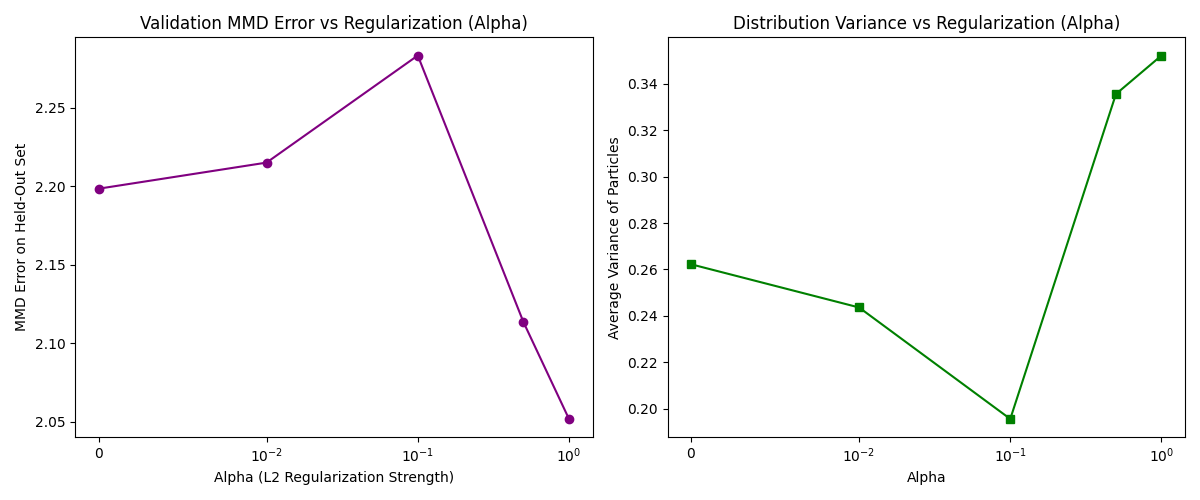
\includegraphics[width=\textwidth]{figures/performance_vs_regularization.png}
    \caption{MMD Error vs. Alpha}
    \label{fig:perf_vs_reg}
\end{subfigure}
\hfill
\begin{subfigure}[b]{0.45\textwidth}
    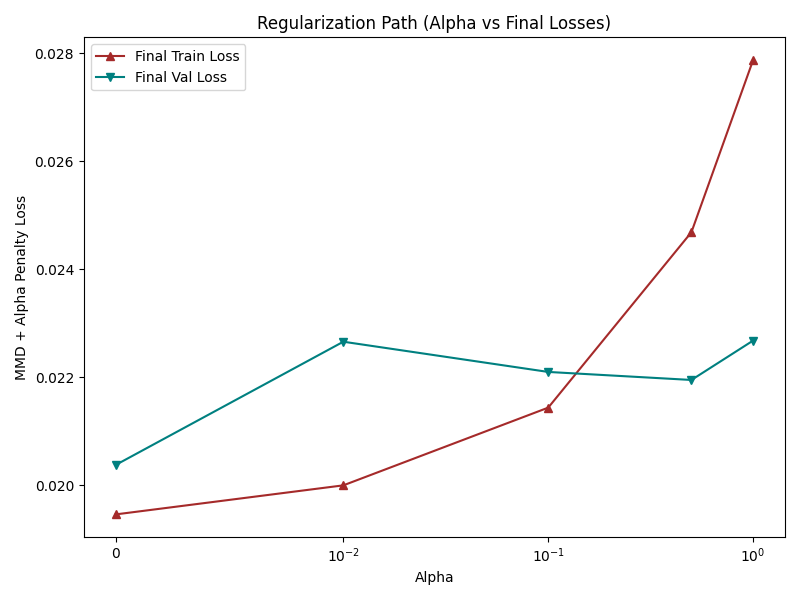
\includegraphics[width=\textwidth]{figures/regularization_path.png}
    \caption{Variance vs. Alpha}
    \label{fig:reg_path}
\end{subfigure}
\caption{Impact of inductive regularization strength ($\alpha$) on distribution matching and expressiveness. Higher $\alpha$ values lead to lower \mmd error and higher variance.}
\label{fig:regularization}
\end{figure}

\subsection{Convergence Analysis}
Training and validation curves (\Figref{fig:curves}) indicate that \immq converges smoothly across all configurations. The \mmd loss declines steadily without the oscillations or explosions often associated with unstructured distributional methods. This stability is attributed to the multi-scale RBF kernel and the inductive bootstrapping process, which together provide a well-behaved gradient signal for the particle updates.

\begin{figure}[h]
\centering
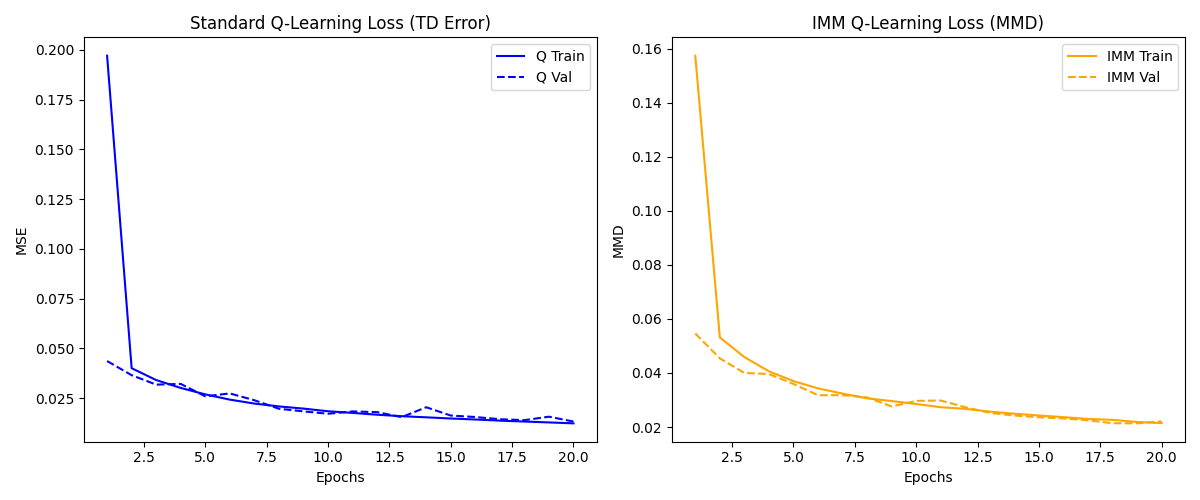
\includegraphics[width=0.7\textwidth]{figures/training_validation_curves.png}
\caption{Training and validation \mmd loss curves for \immq ($\alpha=1.0$, 500 episodes). The smooth decline indicates stable distribution matching.}
\label{fig:curves}
\end{figure}
